\documentclass[aspectratio=169,9pt]{beamer}

% ------------------------------------------------------------
% Theme and typography
% ------------------------------------------------------------
\usetheme{Boadilla}
\usecolortheme{default}
\usepackage[T1]{fontenc}
\usepackage{lmodern}
\usepackage{microtype}
\usepackage{amsmath,amssymb,mathtools}
\usepackage{booktabs,tabularx,array,multirow}
\usepackage{graphicx}
\usepackage{tikz}
\usetikzlibrary{arrows.meta,positioning,fit,calc,shapes.geometric}
\usepackage{ragged2e}
\usepackage{hyperref}
\usepackage{appendixnumberbeamer}

\definecolor{Navy}{HTML}{12304A}
\definecolor{Teal}{HTML}{087E82}
\definecolor{TealLight}{HTML}{E6F4F3}
\definecolor{Gold}{HTML}{D18B23}
\definecolor{GoldLight}{HTML}{FFF4DF}
\definecolor{Ink}{HTML}{243447}
\definecolor{Muted}{HTML}{627487}
\definecolor{Pale}{HTML}{F3F6F9}
\definecolor{Red}{HTML}{B94B48}

\setbeamercolor{normal text}{fg=Ink,bg=white}
\setbeamercolor{structure}{fg=Teal}
\setbeamercolor{frametitle}{fg=Navy,bg=white}
\setbeamercolor{title}{fg=white}
\setbeamercolor{subtitle}{fg=white!85}
\setbeamercolor{author}{fg=white!90}
\setbeamercolor{institute}{fg=white!80}
\setbeamercolor{date}{fg=white!80}
\setbeamercolor{block title}{fg=white,bg=Navy}
\setbeamercolor{block body}{fg=Ink,bg=Pale}
\setbeamercolor{block title alerted}{fg=white,bg=Gold}
\setbeamercolor{block body alerted}{fg=Ink,bg=GoldLight}
\setbeamercolor{block title example}{fg=white,bg=Teal}
\setbeamercolor{block body example}{fg=Ink,bg=TealLight}
\setbeamercolor{item projected}{fg=white,bg=Teal}
\setbeamerfont{frametitle}{series=\bfseries,size=\large}
\setbeamerfont{title}{series=\bfseries,size=\LARGE}
\setbeamertemplate{navigation symbols}{}
\setbeamertemplate{blocks}[rounded][shadow=false]
\setbeamertemplate{itemize item}{\color{Teal}\raise0.25ex\hbox{\small$\blacktriangleright$}}
\setbeamertemplate{itemize subitem}{\color{Gold}\scriptsize$\bullet$}
\setbeamertemplate{frametitle}{%
  \vskip0.35em
  \begin{beamercolorbox}[wd=\paperwidth,ht=1.9ex,dp=0.6ex,leftskip=0.65cm,rightskip=0.4cm]{frametitle}%
    \color{Teal}\rule{2.2pt}{2.0ex}\hspace{0.35em}%
    \insertframetitle
  \end{beamercolorbox}%
  \vspace{-0.15em}\hspace{0.65cm}\color{Teal!35}\rule{\dimexpr\paperwidth-1.3cm\relax}{0.35pt}%
}
\setbeamertemplate{footline}{%
  \leavevmode%
  \hbox{%
  \begin{beamercolorbox}[wd=.72\paperwidth,ht=1.9ex,dp=0.6ex,leftskip=.65cm]{author in head/foot}%
    \color{Muted}\scriptsize NLP CS60075  $\cdot$  Project 5: Static and Contextual Representations
  \end{beamercolorbox}%
  \begin{beamercolorbox}[wd=.28\paperwidth,ht=1.9ex,dp=0.6ex,rightskip=.65cm plus1fil]{date in head/foot}%
    \color{Muted}\scriptsize Yellapu Dheeraj Babu  \hspace{1em} \insertframenumber/\inserttotalframenumber
  \end{beamercolorbox}}%
  \vskip0pt%
}
\setbeamersize{text margin left=0.65cm,text margin right=0.65cm}
\setlength{\leftmargini}{1.25em}
\setlength{\leftmarginii}{1.15em}
\renewcommand{\arraystretch}{1.16}
\graphicspath{{figures/}}

\newcommand{\smallcite}[1]{\vspace{0.15em}{\tiny\color{Muted}#1}}
\newcommand{\metric}[2]{\begin{beamercolorbox}[rounded=true,sep=0.65ex,wd=\linewidth]{block body example}\centering{\Large\bfseries\color{Teal}#1}\\[-0.2ex]{\scriptsize\color{Muted}#2}\end{beamercolorbox}}
\newcommand{\highlight}[1]{\textcolor{Teal}{\bfseries #1}}
\newcommand{\warn}[1]{\textcolor{Red}{\bfseries #1}}
\newcommand{\tightitem}{\setlength{\itemsep}{0.14em}\setlength{\parskip}{0pt}}

\title{From Static to Contextual}
\subtitle{Distributional Semantics and What's Inside BERT}
\author{Yellapu Dheeraj Babu \\ \small 23CS10081}
\institute{NLP CS60075 $\;|\;$ Assignment II -- Project 5 \\ Indian Institute of Technology Kharagpur}
\date{November 2026}

\begin{document}

% ------------------------------------------------------------
% 1. Title
% ------------------------------------------------------------
{\setbeamertemplate{footline}{}
\setbeamertemplate{background canvas}{\color{Navy}\rule{\paperwidth}{\paperheight}}
\begin{frame}[plain]
  \vspace{0.65cm}
  {\color{Teal!35}\rule{1.2cm}{3pt}}\\[0.55cm]
  {\usebeamerfont{title}\color{white}\inserttitle\par}
  \vspace{0.12cm}
  {\usebeamerfont{subtitle}\large\insertsubtitle\par}
  \vspace{0.8cm}
  {\color{white!85}\Large From distributional co-occurrence to contextual syntax\par}
  \vspace{1.05cm}
  {\color{white}\insertauthor\par}
  \vspace{0.2cm}
  {\color{white!80}\insertinstitute\par}
  \vfill
  {\color{white!65}\small 10-minute project presentation \hfill November 2026}
\end{frame}}

% ------------------------------------------------------------
% 2. Motivation
% ------------------------------------------------------------
\begin{frame}{Why compare static and contextual representations?}
\begin{columns}[T,onlytextwidth]
  \column{0.48\textwidth}
  \begin{block}{Static word vectors}
    \centering
    \vspace{0.15em}
    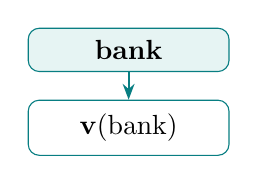
\begin{tikzpicture}[node distance=0.35cm]
      \node[draw=Teal,fill=TealLight,rounded corners,minimum width=2.55cm,minimum height=.55cm] (w) {\textbf{bank}};
      \node[draw=Teal,fill=white,rounded corners,below=of w,minimum width=2.55cm,minimum height=.7cm] (v) {$\mathbf{v}(\text{bank})$};
      \draw[-{Stealth[length=2mm]},thick,Teal] (w)--(v);
    \end{tikzpicture}
    \vspace{0.25em}
    \begin{itemize}\tightitem
      \item One vector per word type.
      \item Meaning is inferred from aggregate co-occurrence.
      \item Efficient, but cannot distinguish a word's different uses.
    \end{itemize}
  \end{block}
  \column{0.48\textwidth}
  \begin{block}{Contextual BERT representations}
    \centering
    \vspace{0.15em}
    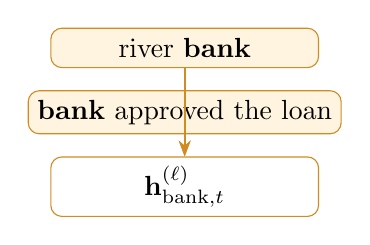
\begin{tikzpicture}[node distance=0.28cm]
      \node[draw=Gold,fill=GoldLight,rounded corners,minimum width=3.4cm,minimum height=.5cm] (s1) {river \textbf{bank}};
      \node[draw=Gold,fill=GoldLight,rounded corners,below=of s1,minimum width=3.4cm,minimum height=.5cm] (s2) {\textbf{bank} approved the loan};
      \node[draw=Gold,fill=white,rounded corners,below=of s2,minimum width=3.4cm,minimum height=.62cm] (v) {$\mathbf{h}_{\text{bank},t}^{(\ell)}$};
      \draw[-{Stealth[length=2mm]},thick,Gold] (s1)--(v);
      \draw[-{Stealth[length=2mm]},thick,Gold] (s2)--(v);
    \end{tikzpicture}
    \vspace{0.25em}
    \begin{itemize}\tightitem
      \item A different vector for each token occurrence.
      \item Encodes left and right sentence context.
      \item Can carry syntax and sense information in its layers.
    \end{itemize}
  \end{block}
\end{columns}
\vspace{0.1em}
\begin{alertblock}{The central question}
Does information useful for word meaning also preserve token-to-token syntax?
\end{alertblock}
\end{frame}

% ------------------------------------------------------------
% 3. Problem statement and project questions
% ------------------------------------------------------------
\begin{frame}{Problem statement and experimental questions}
\begin{block}{Problem statement}
Study the transition from classical static vectors to contextual BERT representations, and test what happens to semantic and syntactic information when contextual vectors are pooled into one vector per word.
\end{block}
\vspace{0.15em}
\begin{columns}[T,onlytextwidth]
  \column{0.32\textwidth}
  \begin{block}{Task 1 -- Baseline}
    \textbf{Build PPMI + SVD vectors.}
    \begin{itemize}\tightitem
      \item Learn from EWT co-occurrence.
      \item Evaluate semantic similarity and analogies.
      \item Check cosine-MST edges against gold trees.
    \end{itemize}
  \end{block}
  \column{0.32\textwidth}
  \begin{block}{Task 2 -- Reproduction}
    \textbf{Probe frozen BERT.}
    \begin{itemize}\tightitem
      \item Learn a linear geometry for tree distance and depth.
      \item Sweep layers and probe ranks.
      \item Select the strongest syntax layer.
    \end{itemize}
  \end{block}
  \column{0.32\textwidth}
  \begin{block}{Task 3 -- Combine and improve}
    \textbf{Pool BERT into static vectors.}
    \begin{itemize}\tightitem
      \item Average the selected layer by word type.
      \item Re-run the same semantic tests.
      \item Compare tree recovery with Task 1.
    \end{itemize}
  \end{block}
\end{columns}
\vspace{0.18em}
\begin{exampleblock}{What is being tested?}
A representation may be good at ranking semantically similar word types without being good at identifying which word tokens are syntactically connected.
\end{exampleblock}
\end{frame}

% ------------------------------------------------------------
% 4. Dataset and evaluation protocol
% ------------------------------------------------------------
\begin{frame}{Dataset and evaluation protocol}
\begin{columns}[T,onlytextwidth]
  \column{0.51\textwidth}
  \begin{block}{UD English EWT}
    \begin{itemize}\tightitem
      \item Web-genre English: reviews, emails, newsgroups, Q\&A and blogs.
      \item Gold Universal Dependencies trees provide token heads for syntax evaluation.
      \item Raw tokens train static vectors; gold heads supply syntax supervision/evaluation.
    \end{itemize}
    \vspace{0.25em}
    \centering
    \begin{tabular}{lrr}
      \toprule
      \textbf{Split} & \textbf{Sentences} & \textbf{Words}\\
      \midrule
      Train & 12,544 & 204,578\\
      Dev & 2,001 & 25,148\\
      Test & 2,077 & 25,094\\
      \bottomrule
    \end{tabular}
  \end{block}
  \column{0.46\textwidth}
  \begin{block}{Evaluation sets and metrics}
    \begin{itemize}\tightitem
      \item \textbf{WordSim-353:} Spearman $\rho$ between model cosine scores and human similarity rankings.
      \item \textbf{Google analogies:} 3CosAdd accuracy; exclude the three query words.
      \item \textbf{Dependency trees:} UUAS after decoding a minimum spanning tree (MST).
      \item \textbf{Structural probe:} depth Spearman alongside UUAS.
    \end{itemize}
  \end{block}
  \vspace{0.1em}\textcolor{Gold}{\textbf{Coverage:}} 248/353 WordSim pairs (70.3\%) and 5,727/19,544 analogy questions (29.3\%) are fully in-vocabulary.
\end{columns}
\smallcite{Dataset splits and fields: UD English EWT, assignment dataset specification and experiment report (November 2026).}
\end{frame}


% ------------------------------------------------------------
% 4b. Code organisation (used for the code walkthrough)
% ------------------------------------------------------------
\begin{frame}[fragile]{Code organisation and how to run}
\begin{columns}[T,onlytextwidth]
  \column{0.52\textwidth}
  \begin{block}{One folder per task}
    \footnotesize
    \begin{tabular}{@{}ll@{}}
      \texttt{code/common/} & data, MST, bootstrap, \textbf{shared evaluation}\\
      \texttt{code/task1/} & co-occurrence $\to$ PPMI $\to$ SVD\\
      \texttt{code/task2/} & BERT features $\to$ probes $\to$ $\ell^*$\\
      \texttt{code/task3/} & pool layer $\ell^*$ $\to$ same evaluation\\
      \texttt{code/run\_all.py} & every step, in order, one log each\\
      \texttt{run\_all\_colab.ipynb} & end-to-end run on Colab\\
    \end{tabular}
  \end{block}
  \begin{exampleblock}{Design choice}
    \footnotesize T1 and T3 call \emph{the same} evaluation function on the same vocabulary, so their comparison uses an identical protocol by construction.
  \end{exampleblock}
  \column{0.45\textwidth}
  \begin{block}{Data flow}
    \centering
    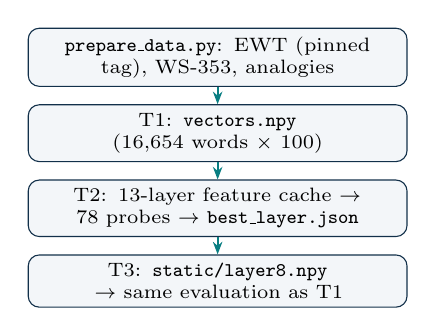
\begin{tikzpicture}[node distance=0.22cm, every node/.style={font=\scriptsize}, b/.style={draw=Navy,rounded corners,fill=Pale,align=center,text width=4.6cm,inner sep=3pt}, a/.style={-{Stealth[length=1.6mm]},thick,Teal}]
      \node[b] (d) {\texttt{prepare\_data.py}: EWT (pinned tag), WS-353, analogies};
      \node[b,below=of d] (t1) {T1: \texttt{vectors.npy} (16,654 words $\times$ 100)};
      \node[b,below=of t1] (t2) {T2: 13-layer feature cache $\to$ 78 probes $\to$ \texttt{best\_layer.json}};
      \node[b,below=of t2] (t3) {T3: \texttt{static/layer8.npy} $\to$ same evaluation as T1};
      \draw[a] (d)--(t1); \draw[a] (t1)--(t2); \draw[a] (t2)--(t3);
    \end{tikzpicture}
  \end{block}
  \vspace{0.1em}
  {\scriptsize\texttt{python code/run\_all.py}\quad$\cdot$\quad seed 42 everywhere}
\end{columns}
\end{frame}

% ------------------------------------------------------------
% 5. Task 1 methodology
% ------------------------------------------------------------
\begin{frame}{Task 1 methodology: PPMI + truncated SVD}
\begin{columns}[T,onlytextwidth]
  \column{0.58\textwidth}
  \begin{enumerate}\tightitem
    \item Count word--context co-occurrences inside each training sentence, using a symmetric window of five words on either side.
    \item Convert raw counts to positive pointwise mutual information:
      \[
        \operatorname{PPMI}(w,c)=\max\!\left(0,\log\frac{P(w,c)}{P(w)P(c)}\right).
      \]
    \item Apply truncated SVD and retain 100 dimensions; use $U\Sigma$ as the word vectors.
    \item Compute cosine similarity for WordSim-353; answer analogies with 3CosAdd:
      \[
        \arg\max_x\;\cos(\mathbf{x},\mathbf{b}-\mathbf{a}+\mathbf{c}).
      \]
  \end{enumerate}
  \column{0.39\textwidth}
  \begin{block}{Structural bonus check}
    For each sampled test sentence:
    \begin{itemize}\tightitem
      \item Compute pairwise cosine distances between word vectors.
      \item Decode an MST using Prim's algorithm.
      \item Compare undirected edges with the gold dependency tree.
    \end{itemize}
    \vspace{0.2em}
    \textbf{Metric:} UUAS = correct undirected edges / gold edges.
  \end{block}
\end{columns}
\vspace{0.25em}
\begin{exampleblock}{Why this is a useful baseline}
PPMI weights above-chance co-occurrence; SVD compresses it. Sparse counts remain the main limitation.
\end{exampleblock}
\end{frame}

% ------------------------------------------------------------
% 6. Task 1 results
% ------------------------------------------------------------
\begin{frame}{Task 1 results: the small training corpus is a bottleneck}
\vspace{-0.1em}
\begin{columns}[T,onlytextwidth]
  \column{0.61\textwidth}
  \begin{block}{Required PPMI-SVD configuration}
    \centering
    \small
    \begin{tabular}{lcc}
      \toprule
      \textbf{Metric} & \textbf{Covered items} & \textbf{All items}\\
      \midrule
      WordSim-353 Spearman $\rho$ & 0.104 & 0.048\\
      Google analogy accuracy & 0.51\% & 0.15\%\\
      MST UUAS (20 sentences) & 20.5\% & --\\
      \bottomrule
    \end{tabular}
  \end{block}
  \begin{itemize}\tightitem
    \item WordSim correlation rises to 0.317 for the 32 covered pairs whose two words occur at least 20 times.
    \item The best tested PPMI variant reaches only $\rho=0.134$; hyperparameter changes do not solve analogy sparsity.
    \item Frequent-word neighbours are often co-occurring partners, but rare-word neighbours are noisy.
  \end{itemize}
  \column{0.36\textwidth}
  \begin{block}{Tree-recovery baselines}
    \metric{20.5\%}{PPMI-SVD, 20-sentence sample}
    \vspace{0.1em}
    \metric{15.2\%}{expected random tree}
    \vspace{0.1em}
    \metric{43.2\%}{linear chain baseline}
  \end{block}
\end{columns}
\begin{alertblock}{Interpretation}
The baseline beats random but trails word order; sparse EWT counts limit lexical estimates and four-word analogies.
\end{alertblock}
\end{frame}

% ------------------------------------------------------------
% 7. Task 2 methodology
% ------------------------------------------------------------
\begin{frame}{Task 2 methodology: a structural probe on frozen BERT}
\vspace{-0.1em}
\begin{columns}[T,onlytextwidth]
  \column{0.48\textwidth}
  \begin{block}{Representations and probe}
    \begin{itemize}\tightitem
      \item Feed each sentence to frozen \texttt{bert-base-uncased}; retain layer 0 (embeddings) and transformer layers 1--12.
      \item Each token has a 768-dimensional representation $\mathbf{h}^{(\ell)}_i$.
      \item Learn $B_\ell\in\mathbb{R}^{k\times768}$ per layer, with $k\in\{32,64,128\}$.
    \end{itemize}
  \end{block}
  \begin{block}{Two geometric objectives}
    \textbf{Tree distance:}
    \[
      d_B(i,j)=\|B_\ell h_i-B_\ell h_j\|_2^2
    \]
    \textbf{Tree depth:}
    \[
      \operatorname{depth}_B(i)=\|B_\ell h_i\|_2^2
    \]
  \end{block}
  \column{0.48\textwidth}
  \begin{block}{Training and decoding}
    \begin{itemize}\tightitem
      \item Gold distances and depths are computed from EWT \texttt{head}.
      \item Train distance and depth probes for every layer/rank.
      \item Adam (initial LR $10^{-3}$), batch 20, 30 epochs; LR $\times0.1$ when dev loss stalls (paper); keep the best dev checkpoint.
      \item Decode an MST from predicted distances.
    \end{itemize}
  \end{block}
  \begin{exampleblock}{Reported measures}
    \textbf{UUAS} evaluates recovered dependency edges; \textbf{depth Spearman} evaluates whether predicted norms rank tokens by gold tree depth.
  \end{exampleblock}
\end{columns}
\end{frame}

% ------------------------------------------------------------
% 8. Task 2 results
% ------------------------------------------------------------
\begin{frame}{Task 2 results: syntax peaks in the middle layers}
\begin{columns}[T,onlytextwidth]
  \column{0.64\textwidth}
    \centering
    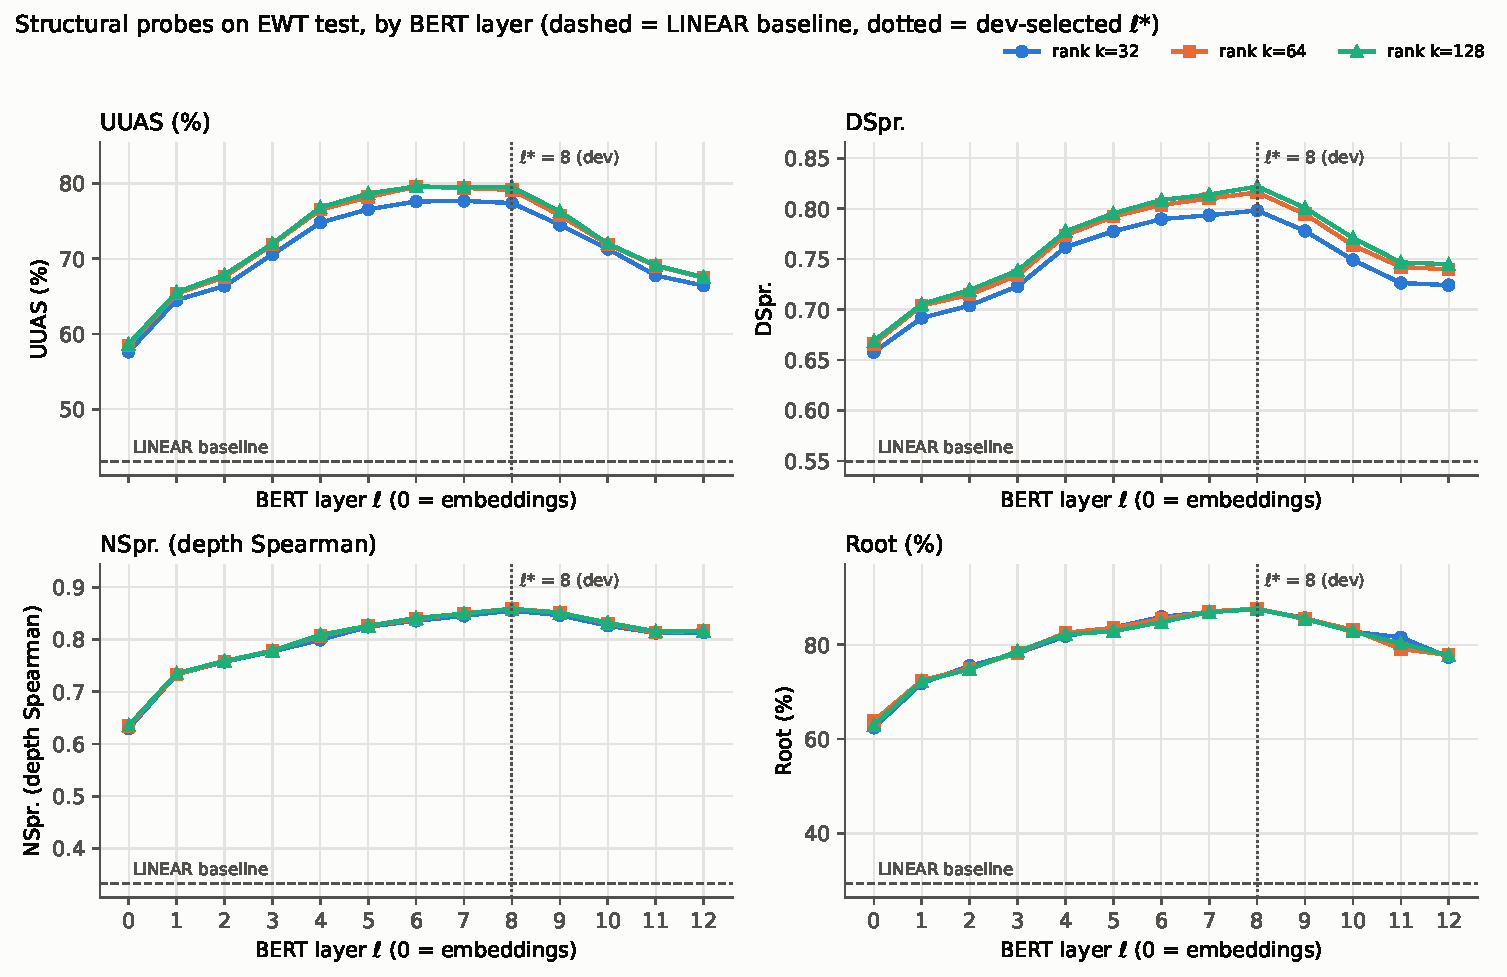
\includegraphics[width=\linewidth,height=4.35cm,keepaspectratio]{metrics_vs_layer.pdf}\par
    \vspace{-0.1em}
    {\tiny UUAS, depth Spearman and root prediction by BERT layer; dotted line marks the dev-selected layer.}
  \column{0.33\textwidth}
    \metric{79.5\%}{test UUAS at layer 8 (paper: 79.8\%)}
    \vspace{0.2em}
    \metric{0.859}{depth Spearman at layer 8 (paper: 0.87)}
    \vspace{0.2em}
    \metric{58.7\% $\rightarrow$ 79.5\%}{layer 0 to layer 8 UUAS}
    \vspace{0.35em}
    \begin{itemize}\tightitem
      \item Layers 6--8 tie statistically; gains saturate by $k=64$.
      \item Layer 12 falls to 67.6\% UUAS.
      \item Paper: PTB/WSJ + cased = 79.8\%; EWT + uncased = 79.5\%.
    \end{itemize}
\end{columns}
\end{frame}

% ------------------------------------------------------------
% 9. Task 3 methodology
% ------------------------------------------------------------
\begin{frame}{Task 3 methodology: turn contextual BERT states into static vectors}
\begin{center}
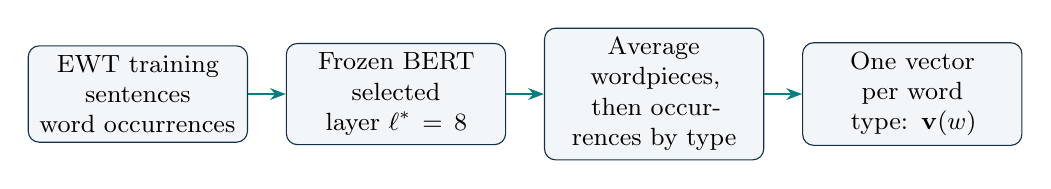
\begin{tikzpicture}[node distance=0.48cm, every node/.style={font=\small}, box/.style={draw=Navy,rounded corners,fill=Pale,align=center,minimum height=.72cm,text width=2.55cm}, arr/.style={-{Stealth[length=2mm]},thick,Teal}]
  \node[box] (sent) {EWT training sentences\\word occurrences};
  \node[box,right=of sent] (bert) {Frozen BERT\\selected layer $\ell^*=8$};
  \node[box,right=of bert] (pool) {Average wordpieces,\\then occurrences by type};
  \node[box,right=of pool] (vec) {One vector per word\\type: $\mathbf{v}(w)$};
  \draw[arr] (sent)--(bert);
  \draw[arr] (bert)--(pool);
  \draw[arr] (pool)--(vec);
\end{tikzpicture}
\end{center}
\vspace{0.25em}
\begin{columns}[T,onlytextwidth]
  \column{0.49\textwidth}
  \begin{block}{Pooling operation}
    For all occurrences $t$ of word type $w$ in EWT train:
    \[
      \mathbf{v}(w)=\frac{1}{N_w}\sum_{t:w_t=w}\mathbf{h}^{(8)}_t.
    \]
    The same lowercased vocabulary and benchmark protocol as Task 1 are used.
  \end{block}
  \column{0.49\textwidth}
  \begin{block}{Post-processing and fairness checks}
    \begin{itemize}\tightitem
      \item Also test all-but-the-top (ABTT): subtract the mean and remove the top 7 principal directions from BERT vectors.
      \item Apply one common evaluation function to T1 and T3.
      \item Reuse the exact same 20 sampled sentences and expanded 660-sentence pool.
    \end{itemize}
  \end{block}
\end{columns}
\begin{alertblock}{Important comparison caveat}
T3 inherits BERT pretraining on roughly 3.3B words; T1 sees only 204.6K EWT words. This is not a same-data comparison.
\end{alertblock}
\end{frame}

% ------------------------------------------------------------
% 10. Task 3 semantic results
% ------------------------------------------------------------
\begin{frame}{Task 3 results: pooled BERT vectors transform semantic performance}
\begin{block}{Comparison: semantic metrics (covered/all) and tree recovery (pool)}
\centering
\small
\begin{tabular}{lccc}
  \toprule
  \textbf{Representation} & \shortstack{\textbf{WordSim $\rho$}\\cov. / all} & \shortstack{\textbf{Analogy (\%)}\\cov. / all} & \shortstack{\textbf{MST UUAS}\\pool}\\
  \midrule
  T1: PPMI-SVD (required) & 0.104 / 0.048 & 0.51 / 0.15 & 24.8\%\\
  T3: BERT-static, layer 8 & 0.577 / 0.452 & 67.7 / 19.8 & 17.9\%\\
  T3 + ABTT & \textbf{0.682 / 0.539} & \textbf{71.0 / 20.8} & 19.6\%\\
  \bottomrule
\end{tabular}
\end{block}
\begin{columns}[T,onlytextwidth]
  \column{0.49\textwidth}
  \begin{exampleblock}{Large semantic gains}
    \begin{itemize}\tightitem
      \item WordSim gain: $+0.474$ for raw T3 and $+0.579$ with ABTT.
      \item ABTT's WordSim gain over T1 has 95\% CI $[0.46,0.71]$.
      \item On analogies, T3 solves 3,848 cases T1 misses; none are solved only by T1 (McNemar $p<10^{-300}$).
    \end{itemize}
  \end{exampleblock}
  \column{0.49\textwidth}
  \begin{block}{Qualitative behaviour}
    \begin{itemize}\tightitem
      \item For \textit{good}, T3 returns \textit{excellent, great, nice, decent, wonderful}.
      \item Strong on plural morphology (96.6\%) and capitals (93.6\%); weak on currency (0/28) and opposites (26.9\%).
    \end{itemize}
  \end{block}
\end{columns}
\vspace{0.1em}
\end{frame}

% ------------------------------------------------------------
% 11. Layer sweep: semantics vs syntax
% ------------------------------------------------------------
\begin{frame}{The best layer depends on what we want to preserve}
\begin{columns}[T,onlytextwidth]
  \column{0.70\textwidth}
    \centering
    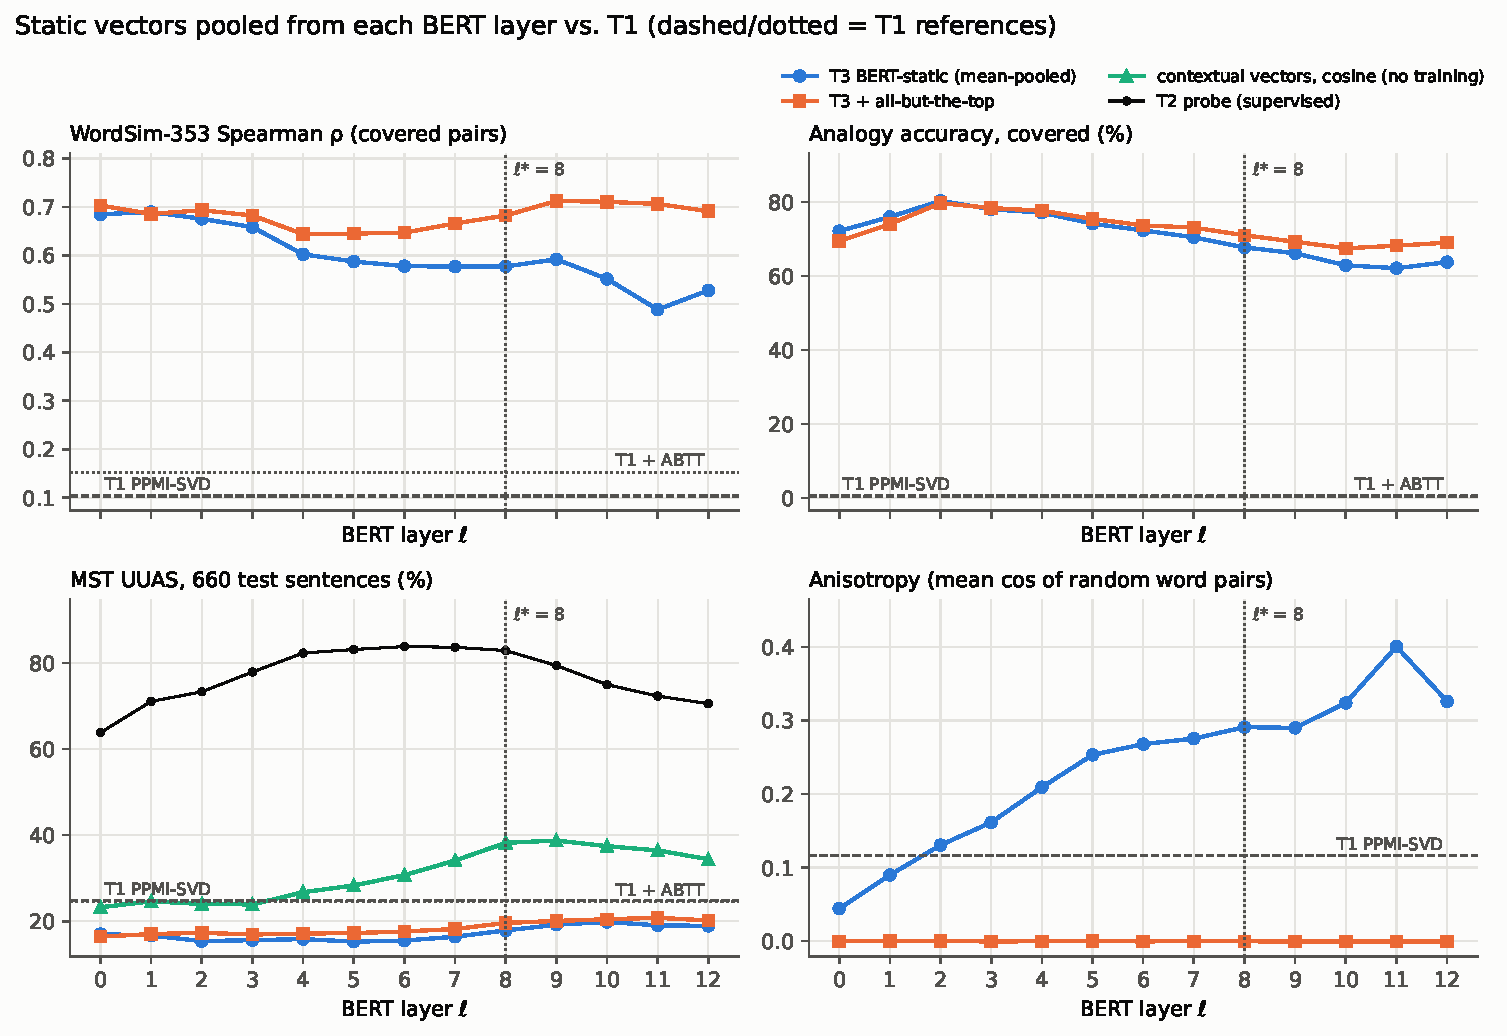
\includegraphics[width=\linewidth,height=4.65cm,keepaspectratio]{layer_sweep.pdf}
  \column{0.28\textwidth}
    \begin{block}{Different optima}
      \begin{itemize}\tightitem
        \item WordSim-353 peaks at layer 1: $\rho=0.690$.
        \item Analogy accuracy peaks at layer 2: 80.3\%.
        \item Syntax probe peaks around layers 6--8; layer 8 is dev-selected.
      \end{itemize}
    \end{block}
    \begin{alertblock}{Why layer 8?}
      It is selected for its syntactic structure, not because it is the best layer for static lexical semantics.
    \end{alertblock}
\end{columns}
\vspace{0.08em}
\smallcite{Layer-wise analysis is from the experiment report; contextual-to-static layer trends are consistent with Bommasani et al. (ACL 2020).}
\end{frame}

% ------------------------------------------------------------
% 12. Task 3 structural results
% ------------------------------------------------------------
\begin{frame}{Task 3 results: semantic gains do not transfer to tree recovery}
\begin{columns}[T,onlytextwidth]
  \column{0.62\textwidth}
    \centering
    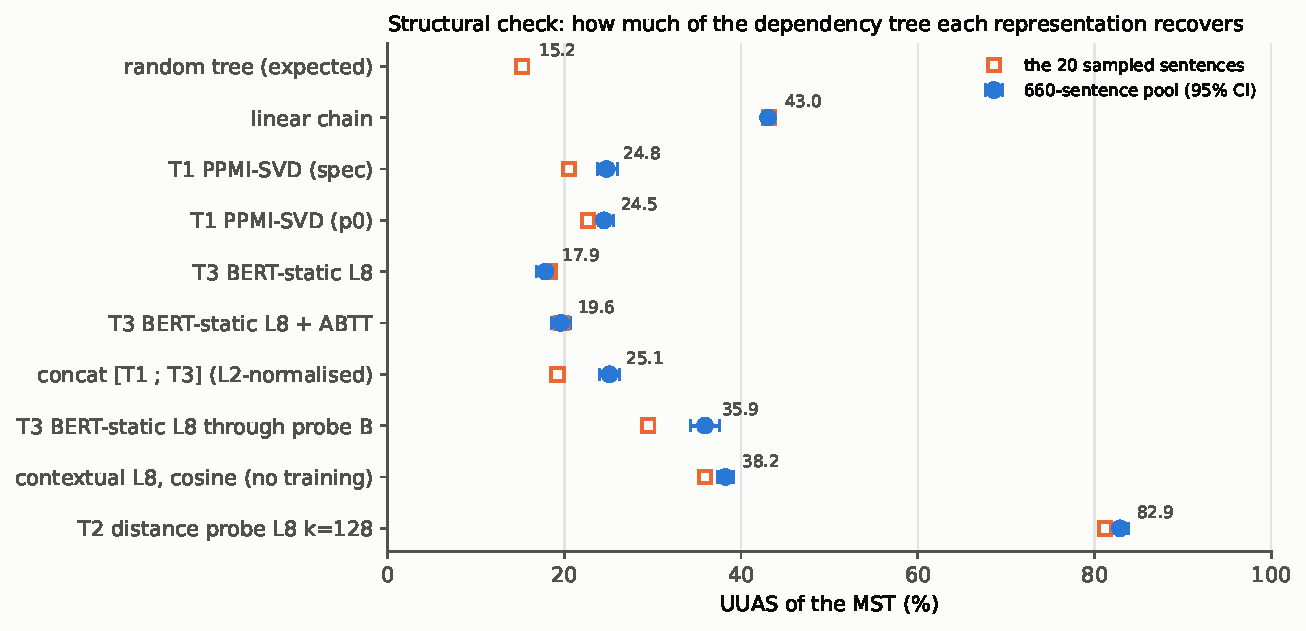
\includegraphics[width=\linewidth,height=4.05cm,keepaspectratio]{ladder.pdf}
  \column{0.35\textwidth}
    \begin{block}{660-sentence pool}
      \begin{tabular}{lr}
        \toprule
        Representation & UUAS\\
        \midrule
        Random tree & 17.1\%\\
        T3 static, layer 8 & 17.9\%\\
        T3 + ABTT & 19.6\%\\
        T1 PPMI-SVD & 24.8\%\\
        Contextual cosine & 38.2\%\\
        Linear chain & 43.0\%\\
        T2 structural probe & \textbf{82.9\%}\\
        \bottomrule
      \end{tabular}
    \end{block}
\end{columns}
\vspace{0.1em}
\begin{beamercolorbox}[rounded=true,sep=0.65ex,wd=\linewidth]{block body example}
  \small \textbf{Takeaway:} The 20-sentence T1--T3 difference is not significant; on the 660-sentence pool T3 is 6.9 points below T1 (95\% CI $[-8.0,-5.8]$). The probe reaches 82.9\% by learning syntax-specific token geometry.
\end{beamercolorbox}
\end{frame}

% ------------------------------------------------------------
% 13. Why they disagree
% ------------------------------------------------------------
\begin{frame}{Why the evaluations disagree: substitutes are not syntactic partners}
\begin{columns}[T,onlytextwidth]
  \column{0.49\textwidth}
  \begin{block}{Paradigmatic similarity: T3}
    \begin{itemize}\tightitem
      \item 74.0\% of T3 top-10 neighbours share its majority POS (T1: 32.6\%).
      \item Example: \textit{car} $\rightarrow$ \textit{cars, vehicle, vehicles, SUV, Ferrari}.
      \item These substitutes help lexical similarity.
    \end{itemize}
  \end{block}
  \begin{block}{Syntagmatic association: T1}
    \begin{itemize}\tightitem
      \item T1 neighbours co-occur within $\pm5$ tokens 55.7\% of the time (T3: 16.2\%).
      \item Example: \textit{car} $\rightarrow$ \textit{home, guy, test, driving, drive}.
      \item Co-occurrence can reflect sentence-level partners.
    \end{itemize}
  \end{block}
  \column{0.48\textwidth}
  \begin{block}{Direct structural diagnostics}
    \small
    \begin{tabular}{lcc}
      \toprule
      \textbf{Diagnostic} & \textbf{T1} & \textbf{T3}\\
      \midrule
      Gold edge closer than non-edge (AUC) & 0.54 & 0.46\\
      Function-word mean MST degree & 1.84 & 2.29\\
      Same-UPOS nearest neighbours & 0.33 & 0.74\\
      \bottomrule
    \end{tabular}
  \end{block}
  \begin{alertblock}{Mechanism}
    Averaging retains dictionary-like meaning but removes which head or dependent a particular token attaches to.
  \end{alertblock}
\end{columns}
\end{frame}

% ------------------------------------------------------------
% 14. Qualitative example
% ------------------------------------------------------------
\begin{frame}{A sentence-level example makes the loss visible}
\begin{columns}[T,onlytextwidth]
  \column{0.55\textwidth}
    \centering
    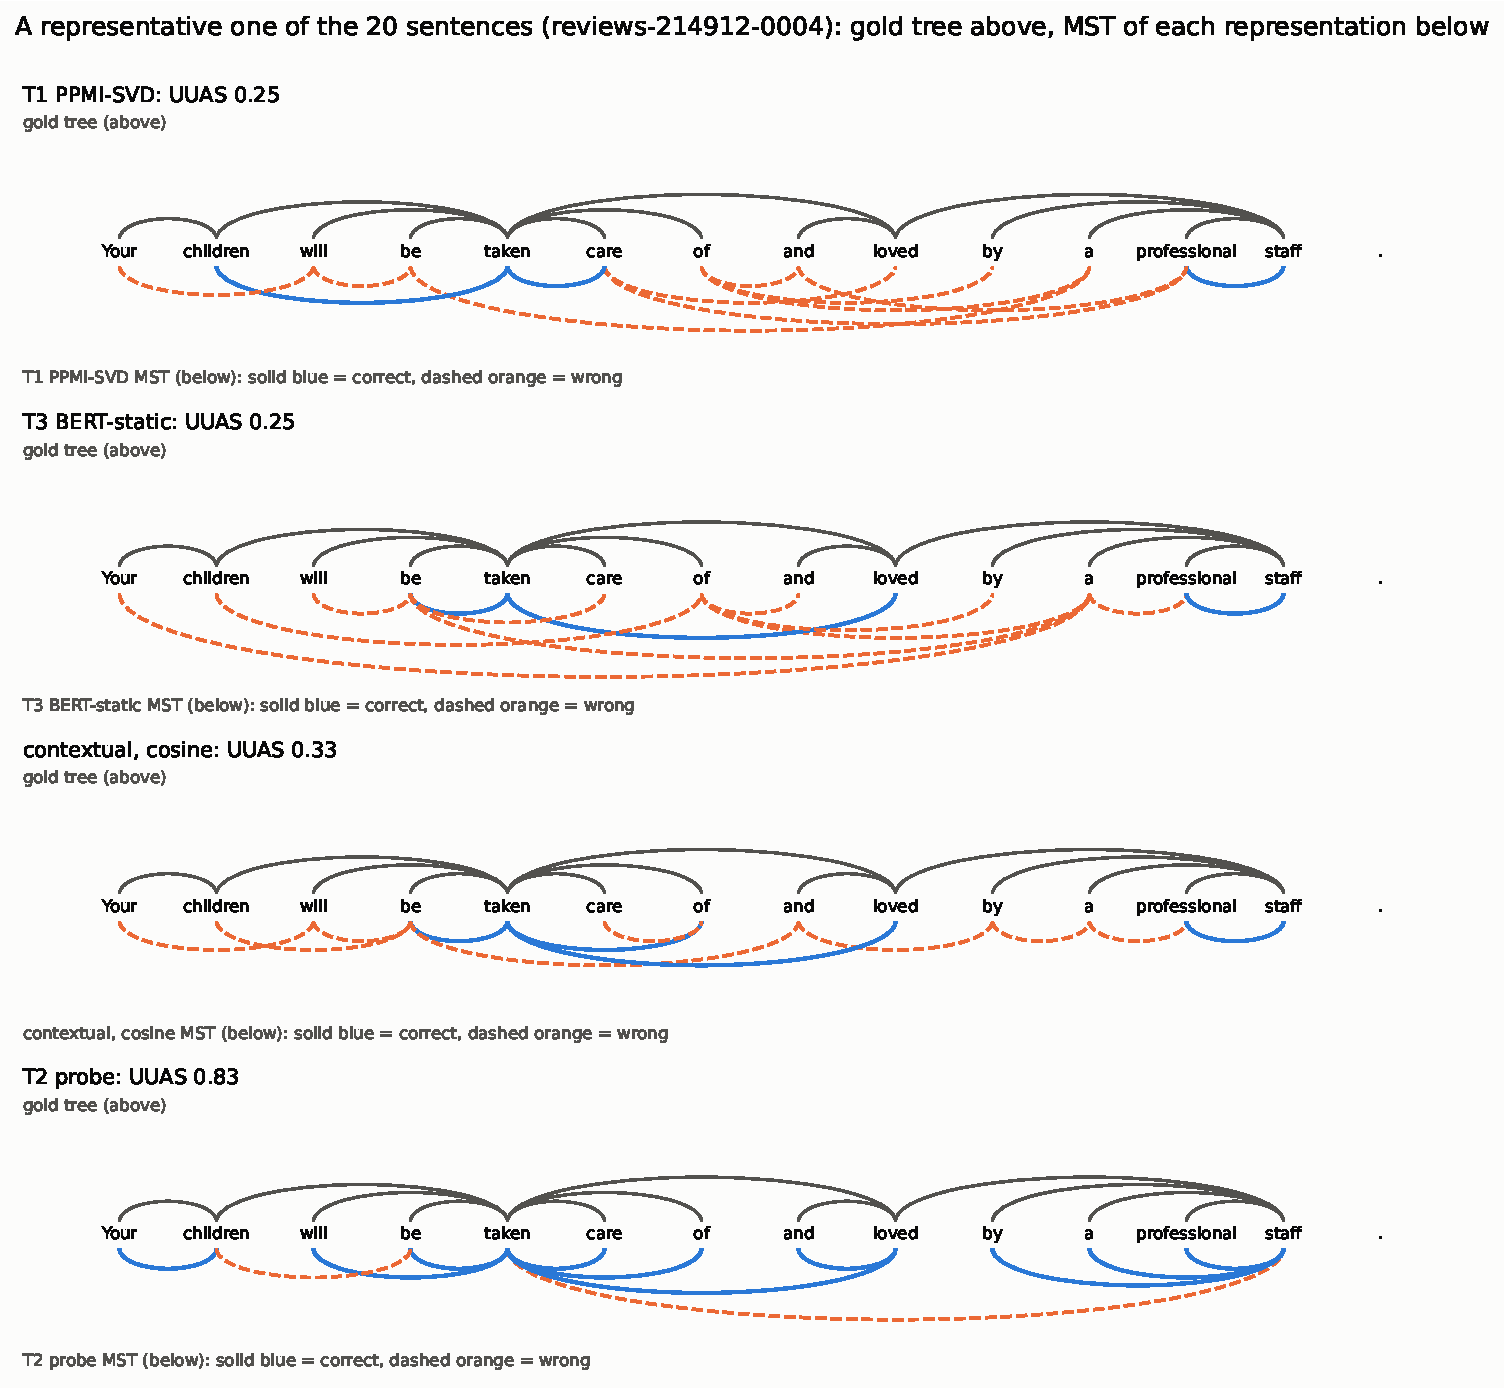
\includegraphics[width=\linewidth,height=4.75cm,keepaspectratio]{mst_example.pdf}
  \column{0.42\textwidth}
    \begin{block}{Example sentence}
      \small\textit{``Your children will be taken care of and loved by a professional staff.''}
    \end{block}
    \begin{itemize}\tightitem
      \item T1 PPMI-SVD: 25\% UUAS.
      \item T3 BERT-static layer 8: 25\% UUAS.
      \item Raw contextual cosine: 33\% UUAS.
      \item T2 trained structural probe: \textbf{83\% UUAS}.
    \end{itemize}
    \begin{alertblock}{What to notice}
      Pooled vectors produce long, incorrect links; the learned probe recovers more gold edges through a syntax-aligned projection.
    \end{alertblock}
\end{columns}
\vspace{0.05em}
\smallcite{Representative sentence selected as the example whose per-method scores were closest to each method's average among the 20 sampled sentences.}
\end{frame}

% ------------------------------------------------------------
% 15. Reproducibility, deviations, limitations
% ------------------------------------------------------------
\begin{frame}{Reproducibility, protocol deviations and limitations}
\begin{columns}[T,onlytextwidth]
  \column{0.49\textwidth}
  \begin{block}{Reproducibility controls}
    \begin{itemize}\tightitem
      \item Seed 42 for sampling, SVD, bootstraps and experiments.
      \item UD 2.18 loader tag; BERT checkpoint \texttt{bert-base-uncased}, revision \texttt{86b5e09}.
      \item Python 3.12, PyTorch 2.15, Transformers 5.22, Datasets 5.1; 2 NVIDIA L40S GPUs.
      \item Runtime: BERT features 7 min; 78 probes about 49 + 54 min on two GPUs.
    \end{itemize}
  \end{block}
  \column{0.49\textwidth}
  \begin{block}{Important deviations and checks}
    \begin{itemize}\tightitem
      \item Probe used learning-rate decay and best-dev selection, following the paper.
      \item Constant $10^{-3}$ LR / epoch-30 control retains layer 8 but reaches only 62.0\% UUAS (non-convergence).
      \item Layer 0 is the non-contextual baseline; 660 sentences supplement the required 20-sentence sample.
    \end{itemize}
  \end{block}
\end{columns}
\begin{alertblock}{Limitations}
One treebank and one BERT model; unequal pretraining resources; a selected in-vocabulary sentence pool; and an under-powered 20-sentence check. Causes of the small paper gap are plausible, not isolated.
\end{alertblock}
\end{frame}

% ------------------------------------------------------------
% 16. Conclusions
% ------------------------------------------------------------
\begin{frame}{Conclusions: what did the experiments establish?}
\begin{enumerate}\tightitem
  \item \textbf{Classical distributional vectors are data-hungry.} PPMI-SVD trained on 204.6K EWT words provides only weak semantic benchmarks and limited tree recovery.
  \item \textbf{BERT contains recoverable syntax.} A linear structural probe reaches 79.5\% UUAS on EWT test, with the strongest geometry around layers 6--8.
  \item \textbf{Pooling helps lexical semantics, not syntax.} Layer-8 BERT-static vectors raise WordSim-353 correlation from 0.104 to 0.577 (0.682 with ABTT), but reduce pool UUAS from 24.8\% to 17.9\%.
  \item \textbf{The objectives are different.} Semantic benchmarks reward paradigmatic similarity between word types; dependency recovery needs token-specific, syntagmatic relations in context.
\end{enumerate}
\vspace{0.35em}
\begin{beamercolorbox}[rounded=true,sep=1.0ex,wd=\linewidth]{block body example}
  \centering\Large\bfseries\color{Navy}
  A good static meaning vector is not automatically a good syntactic representation.
\end{beamercolorbox}
\vspace{0.3em}
\centering\Large\color{Teal}\textbf{Thank you}\quad\textcolor{Muted}{\normalsize Questions?}
\end{frame}

% ------------------------------------------------------------
% 17. References
% ------------------------------------------------------------
\begin{frame}{Selected references}
\footnotesize
\begin{columns}[T,onlytextwidth]
  \column{0.49\textwidth}
  \begin{itemize}\setlength{\itemsep}{0.55em}
    \item Z. S. Harris (1954). \textit{Distributional structure}. \textit{Word}, 10(2--3).
    \item J. Devlin, M.-W. Chang, K. Lee, K. Toutanova (2019). \textit{BERT: Pre-training of deep bidirectional transformers for language understanding}. NAACL-HLT. \href{https://doi.org/10.18653/v1/N19-1423}{doi:10.18653/v1/N19-1423}.
    \item O. Levy and Y. Goldberg (2014). \textit{Neural word embedding as implicit matrix factorization}. NeurIPS. \href{https://papers.neurips.cc/paper/5477-neural-word-embedding-as-implicit-matrix-factorization}{paper}.
    \item J. Hewitt and C. D. Manning (2019). \textit{A structural probe for finding syntax in word representations}. NAACL-HLT, 4129--4138. \href{https://doi.org/10.18653/v1/N19-1419}{doi:10.18653/v1/N19-1419}.
  \end{itemize}
  \column{0.49\textwidth}
  \begin{itemize}\setlength{\itemsep}{0.55em}
    \item R. Bommasani, K. Davis, C. Cardie (2020). \textit{Interpreting pretrained contextualized representations via reductions to static embeddings}. ACL, 4758--4781. \href{https://doi.org/10.18653/v1/2020.acl-main.431}{doi:10.18653/v1/2020.acl-main.431}.
    \item J. Mu and P. Viswanath (2018). \textit{All-but-the-top: Simple and effective postprocessing for word representations}. ICLR.
    \item M. Sahlgren (2006). \textit{The Word-Space Model}. Ph.D. thesis, Stockholm University.
    \item M.-C. de Marneffe, C. D. Manning, J. Nivre, D. Zeman (2021). \textit{Universal Dependencies}. \textit{Computational Linguistics}, 47(2).
  \end{itemize}
\end{columns}
\vspace{0.5em}
\begin{beamercolorbox}[rounded=true,sep=0.8ex,wd=\linewidth]{block body}
  \scriptsize Numerical results, experiment settings, plots and qualitative examples are from the supplied Project 5 report and its generated tables/figures. Assignment framing and dataset requirements follow the supplied CS60075 Project 5 and UD English EWT dataset specifications.
\end{beamercolorbox}
\end{frame}

\end{document}
